\documentclass{article} \usepackage{aaai} \usepackage{graphicx}

% Big margins for now so people can take notes/scribbles.
%\usepackage{fullpage}

\title{Parallel Best NBlock First}
\author{Ethan Burns \and Seth Lemons \and Wheeler Ruml \\
Department of Computer Science \\
University of New Hampshire \\
Durham, NH 03824 USA \\
\{eaburns,seth.lemons, ruml\}@unh.edu}
\date{\today}

\begin{document}
\maketitle

\begin{abstract}
We are approaching a time when it will no longer be beneficial for
hardware manufactures to create micro-processors with greater clock
speeds.  In order to get increased performance, software developers
will need to take advantage of concurrency and multi-core processors.
We make use of novel ideas used for external memory search to create a
parallel best-first-ish algorithm for quickly solving problems which
are small enough to fit into memory.
\end{abstract}

\section{Introduction}

As microprocessor manufacturers build processors with more and more
cores, software developers are being pressured to create algorithms to
make better use of the newly available parallelism.

\section{Previous Work}

\subsection{Structured Duplicate Detection}

Structured Duplicate Detection or SDD \cite{zhou:sdd} is a method for
performing external memory search.  SDD uses a projection function,
which is a many-to-one mapping from states in the search space to
states in an abstract space, to decompose a search graph.  The
projection function creates an abstract space of nodes that are
projections, or images, of the nodes in the original state space.  For
a projection function $p$, $y$ is said to be the \emph{image} of a
node $x$ if $p(x) = y$.  Additionally $y'$ is a successor of $y$, in
the abstract graph, if there are two states $x$ and $x'$ such that
$x'$ is a successor of $x$, $y$ is the image of $x$ and $y'$ is the
image of $x'$.  In other words:

\begin{eqnarray*}
&&x' \in successors(x) \wedge p(x) = y \wedge p(x') = y' \\
&\Rightarrow& y' \in successors(y)
\end{eqnarray*}

In the description of the SDD algorithm, Zhou and Hansen use the term
\emph{nblock} to refer to all nodes in the original state space that
have the same image in the abstract space, throughout the remainder of
this paper, the terms ``abstract state'', and ``nblock'' will be used
interchangeably since each nblock corresponds to a single abstract
state.

Zhou and Hansen show that, while performing duplicate detection, only
nodes which reside within the same nblock must be checked for
duplicates.  By the definition of the successor set of an abstract
node: any child node $x'$ of a node $x$, in the original state space,
will have an image $p(x') \in successors(p(x))$, and therefore when
performing duplicate detection for $x'$ the only nodes that must be
checked are in the nblock $p(x') \in successors(p(x))$.  For this
reason, $successors(p(x))$ is called the \emph{duplicate detection
  scope} of the nblock $p(x)$ -- no other nodes in the original state
space will ever need to be consulted for duplicate detection when
expanding nodes in the nblock $p(x)$.

This idea can be shown using the sliding tile puzzle as an example.
It is conceivable that a projection function for the sliding tiles
puzzle would be to only look at the position of the empty tile.  For
example: all states with the empty tile in the upper left-hand corner
(position 0) would map to the nblock shown in Figure
\ref{fig:tile-abstraction}, where the grayed square represents the
position of the empty tile.  Using this abstraction, there are sixteen
possible abstract states (one for each possible position of the empty
tile).  It is easy to see that all of the children of a state in the
nblock shown in Figure \ref{fig:tile-abstraction} will have the empty
tile in either position 1 or 4 (either by sliding the tile in position
1 to the left, or by sliding the tile in position 4 up).  Figure
\ref{fig:duplicate-detection-scope} shows the duplicate detection
scope for the nblock in Figure \ref{fig:tile-abstraction}.  Any of the
children of a state in the nblock shown in Figure
\ref{fig:tile-abstraction} will fall into one of the two nblocks shown
in Figure \ref{fig:duplicate-detection-scope}.

\begin{figure}[t]
\begin{center}
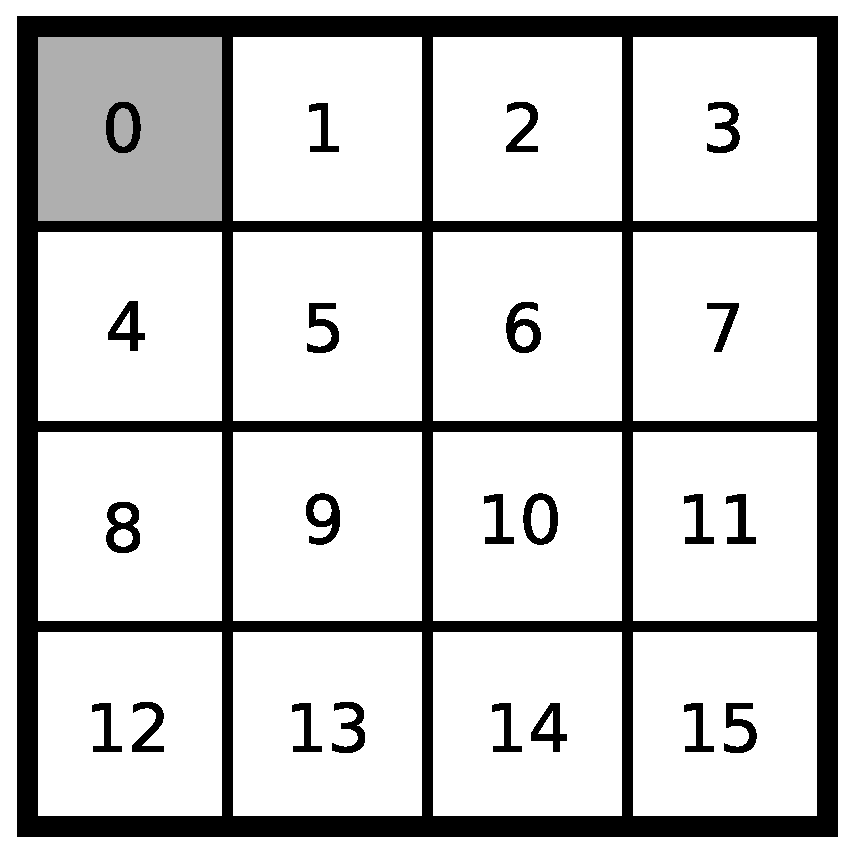
\includegraphics[width=1.5in]{images/tile-abstraction.eps}
\caption{The abstract image of all states with a empty tile in
  position 0.}
\label{fig:tile-abstraction}
\end{center}
\end{figure}

\begin{figure}[t]
\begin{center}
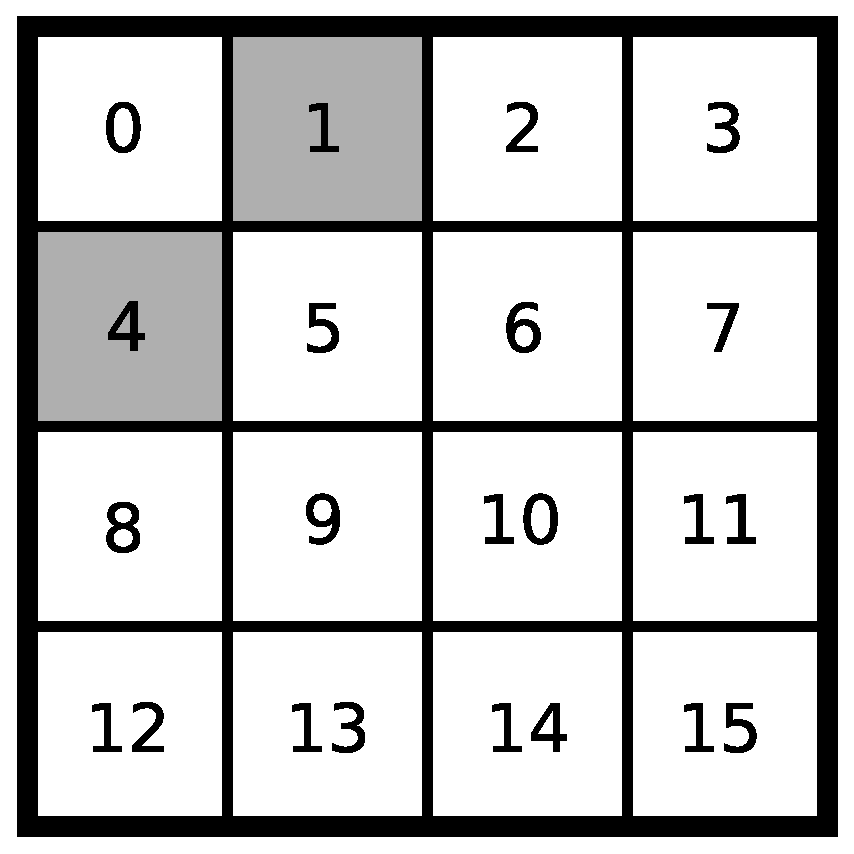
\includegraphics[width=1.5in]{images/duplicate-detection-scope.eps}
\caption{The duplicate detection scope of the abstract node shown in
  Figure \ref{fig:tile-abstraction}.}
\label{fig:duplicate-detection-scope}
\end{center}
\end{figure}

The main focus of the SDD approach is using state space decomposition
so that generated nodes can be explicitly moved to a secondary storage
device (such as a disk drive) when they are not needed.  The SDD
approach uses breadth-first heuristic search, where only the nodes of
the current search depth in a single nblock are searched at a time.
Nodes of this nblock are expanded from the current depth-layer and
their children are placed into the next-depth layer of their
corresponding nblocks.  When the current nblock has no more nodes at
the current depth-layer, it is swapped for another nblock which does
have open nodes at this depth.  If no more nblocks have nodes at the
search depth, the search progresses to the next layer (which contains
the children nodes of the previous layer).  This procedure repeats
until a goal is found, or no nodes remain. Since duplicates can only
fall into the duplicate detection scope of the nblock being searched,
the remainder of the nodes can be pushed off to disk, instead of being
stored in main-memory.  Nblocks can then be intelligently swapped into
and out of main-memory as the search progresses.

\subsection{Parallel Structured Duplicate Detection (PSDD)}

While the motivation of SDD is to have explicit control over which
portions of a search space reside in main-memory.  Zhou and Hansen
also show that this approach also lends itself to parallelization
\cite{zhou:psd}.  The parallel SDD (or PSDD) algorithm uses the graph
of nblocks to find \emph{disjoint duplicate detection scopes}, or
duplicate detection scopes that do not overlap.  Nblocks with disjoint
duplicate detection scopes can be searched in parallel without any
locking or contention.  In order to find nblocks with disjoint
duplicate detection scopes the concept of a \emph{free} nblock is
introduced.  An nblock $b$ is considered to be free if no processor is
using an nblock in $successors(b)$ -- in other words, if all other
processors are searching nblocks with duplicate detection scopes which
are disjoint from that of $b$.  Free nblocks are found by tracking a
$\sigma(b)$ value for each nblock $b$, where $\sigma(b)$ is the number
of nblocks in $successors(b)$ that are in use by another processor.
Any nblock $b$ with $\sigma(b) = 0$ is free, and therefore a processor
can acquire $b$ and its duplicate detection scope for a period of lock
free expansion.  Besides tracking disjoint duplicate detection scopes,
the search procedure of PSDD is the same as that of SDD; the search
progresses by searching one depth-layer at a time until a goal is
found or the search space is exhausted.  PSDD is an attractive
algorithm because it reduces the amount of contention between
processors by allowing for lock-free periods of expansion.

\subsection{Localizing A*}

An alternative approach for improving the efficiency of large searches
is to slightly loosen the node ordering restriction of A* as is done
by Edelkamp and Schrodl \cite{edelkamp:loc}.  Edelkamp and Schrodl
create an algorithm that loosens the node ordering of A* in order to
achieve a better memory locality, this algorithm will be called lA*
(for localized A*).  While lA* expands more nodes than A* does, the
intuition is that lA* can achieve better performance than A* for large
searches because it can reduce the number of virtual-memory operations
that swap to disk.

lA* uses a data structure called a \emph{Heap-of-heaps} to order its
node expansions.  A heap-of-heaps, $H$, is composed of elements $H_0$,
$H_1$, ..., $H_n$, where each element $H_i$ is a heap of search nodes
that reside in the same page of memory.  The heap-of-heaps, $H$, is
loosely sorted based on the f-values of the best nodes of each heap
$H_i$ (denoted as $best(H_i)$).  The lA* procedure searches the best
heap $H_0$, of the heap-of-heaps, until $best(H_1) + \Delta >
best(H_0)$, where $H_1$ is the new best heap on $H$ after the removal
of heap $H_0$.  The $\Delta$ value allows the search to expand a set
of nodes in $H_0$ which may not have a the best f-values, but that
have better memory locality with respect to the previously expanded
nodes.

Since lA* prefers nodes with better memory locality, it reduces the
number of page-faults, and virtual memory swap operations that the
operating system must perform.  The tradeoff is that the first
solution found by lA* may be sub-optimal, since it is not searching in
strict f-value order.  To fix this problem, lA* doesn't return its
first solution; instead it behaves like an any-time algorithm and
continues the search, pruning on the f-value of the incumbent
solution.  Since the f-value of the incumbent solution is an
upper-bound on the optimal solution, the search can stop when there
are no frontier nodes that have f-values less than the current
incumbent -- this means that the current incumbent solution \emph{is}
the optimal solution.

\section{Parallel Best NBlock First (PBNF)}
\subsection{Safe PBNF}
\section{Experimental Results}
\section{Conclusion}

\bibliography{master}
\bibliographystyle{aaai}

\end{document}
